\section{GUI}
\label{gui}

\begin{figure}[H]
    \begin{center}
    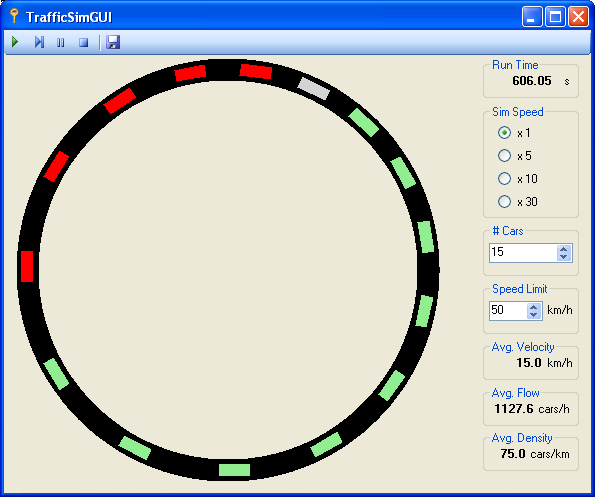
\includegraphics[width=1\textwidth]{simulator2.png}
    \caption{Graphical interface of the simulator which is programmed in C\#. In this figure the road is 200m long with 15 cars. Red cars are braking, green cars are accelerating and the grey car is keeping a constant speed.}
    \end{center}
\end{figure}

\section{Results}
\label{app_postime_plot}
\begin{figure}[H]
    \begin{center}
    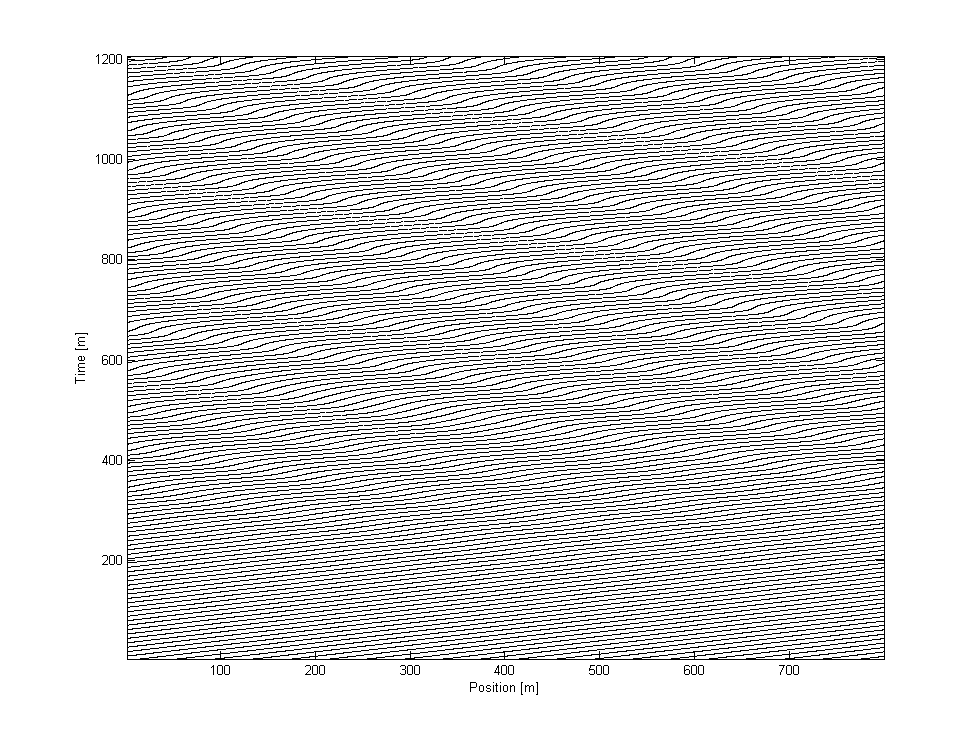
\includegraphics[width=1\textwidth]{acc_60cars_50kmh.png}
    \caption{\label{acc_postime}
Absolute position of 60 cars equipped with adaptive cruise control during $ 1200
\unit{s} $. Data from simulator. After $ 400 \unit{s} $ phantom jams were emerging.}
    \end{center}
\end{figure}

\begin{figure}[H]
    \begin{center}
    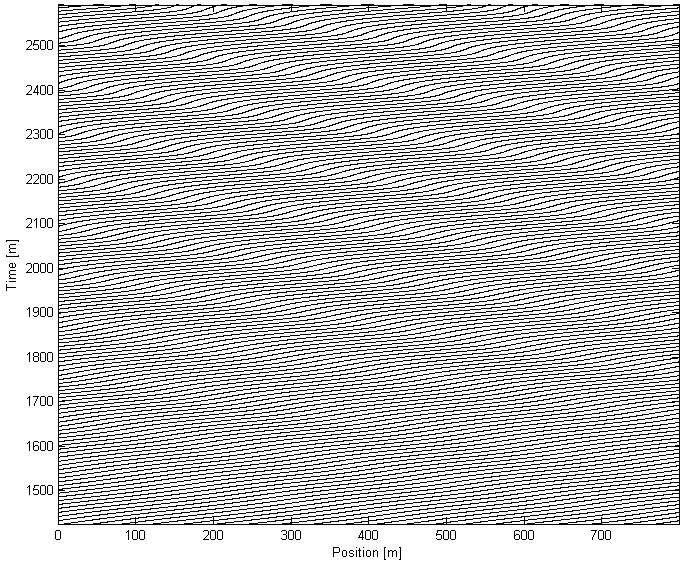
\includegraphics[width=1\textwidth]{eacc_60cars_50kmh.png}
    \caption{\label{eacc_postime}
Absolute position of 60 cars equipped with enhanced adaptive cruise control in
the timegep $ 1200 - 2600 \unit{s} $. Data from simulator. After $ 1300 \unit{s}
$ phantom jams were emerging.}
    \end{center}
\end{figure}
